\chapter*{Quelques Grandeurs Utiles}

\section{Constantes physiques}
\begin{itemize}
\item vitesse de la lumière $c=2.99792458 \times 10^8$ m/s
\item constante de Newton $G=6.6726 \times 10^{-11}$ m$^3$/kg/s$^2$
\item constante de Planck réduite $\hbar = 1.054572\times 10^{-34}$ J s
\item constante de Boltzmann $k_B=1.3806 \times 10^{-23}$ J/K
\end{itemize}

\section{Masses}
\begin{itemize}
\item masse de l'électron $m_e=9.109\times10^{-31}$ kg
\item masse du proton $m_p=1.672\times10^{-27}$ kg
\item masse du neutron $m_n=1675\times10^{-27}$ kg
\item masse du Soleil $M_\odot=1.989\times 10^{30}$ kg
\end{itemize}

\section{Distances}
\begin{itemize}
\item parsec 1 pc = $3.0856\times 10^{16}$ m
\item Mégaparsec 1 Mpc = $10^6\mathrm{pc}=3.0856\times 10^{22}$ m
\item Gigaparsec 1 Gpc = $10^9\mathrm{pc}=3.0856\times 10^{25}$ m
\end{itemize}

\section{Énergies}
\begin{itemize}
\item luminosité du Soleil $L_\odot=3.9\times 10^{26}$ W
\item électron-volt 1 eV=$1.6022\times 10^{-19}$ J 
\item erg 1 erg=$10^{-7}$ J
\item unité naturelle de température 1 MeV=$1.1605\times 10^{10}$ K
\item unité naturelle de masse 1 MeV=$1.783\times10^{-30}$ kg
\end{itemize}

\section{Quantités Cosmologiques}
\begin{itemize}
\item paramètre de Hubble réduit $h=H_0/100\mathrm{km/s/Mpc}$
\item temps de Hubble $H_0^{-1}=9.7776 \times 10^9 h^{-1}$ années
\item densité de l'Univers $\rho=1.8789\times 10^{-26} \Omega_m h^2$ kg/$m^3$
\item densité d'atomes d'hydrogène $n_H=8.42\Omega_b h^2$ m$^{-3}$
\end{itemize}


\section{Planck 2015}
Quantités extraites de \textit{Planck Collaboration 2016, A\& A, 594, A13 (Paper XIII), Table 4 (TT, TE, EE + lowP + lensing + ext)}
\begin{itemize}
\item densité de matière $\Omega_m=0.3075$
\item densité d'énergie noire $\Omega_\Lambda = 0.691$
\item densité de photons $\Omega_\gamma = 5.39 \times 10^{-5}$
\item densité de neutrinos $\Omega_\nu = 0.0014$
\item densité de baryons $\Omega_b=0.0486$
\item paramètre de Hubble $H_0=67.74$ km/s/Mpc
\item âge de l'Univers $t_0=13.798$ milliards d'années
\item température du fond diffus de photons $T_0=2.7255$ K
\item température du fond diffus de neutrinos $T_{\nu0}=1.9454$ K
\item densité critique $\rho_c=8.619\times 10^{-30}$ g/cm$^3$
\end{itemize}

\begin{figure}[htbp]
	\centering
		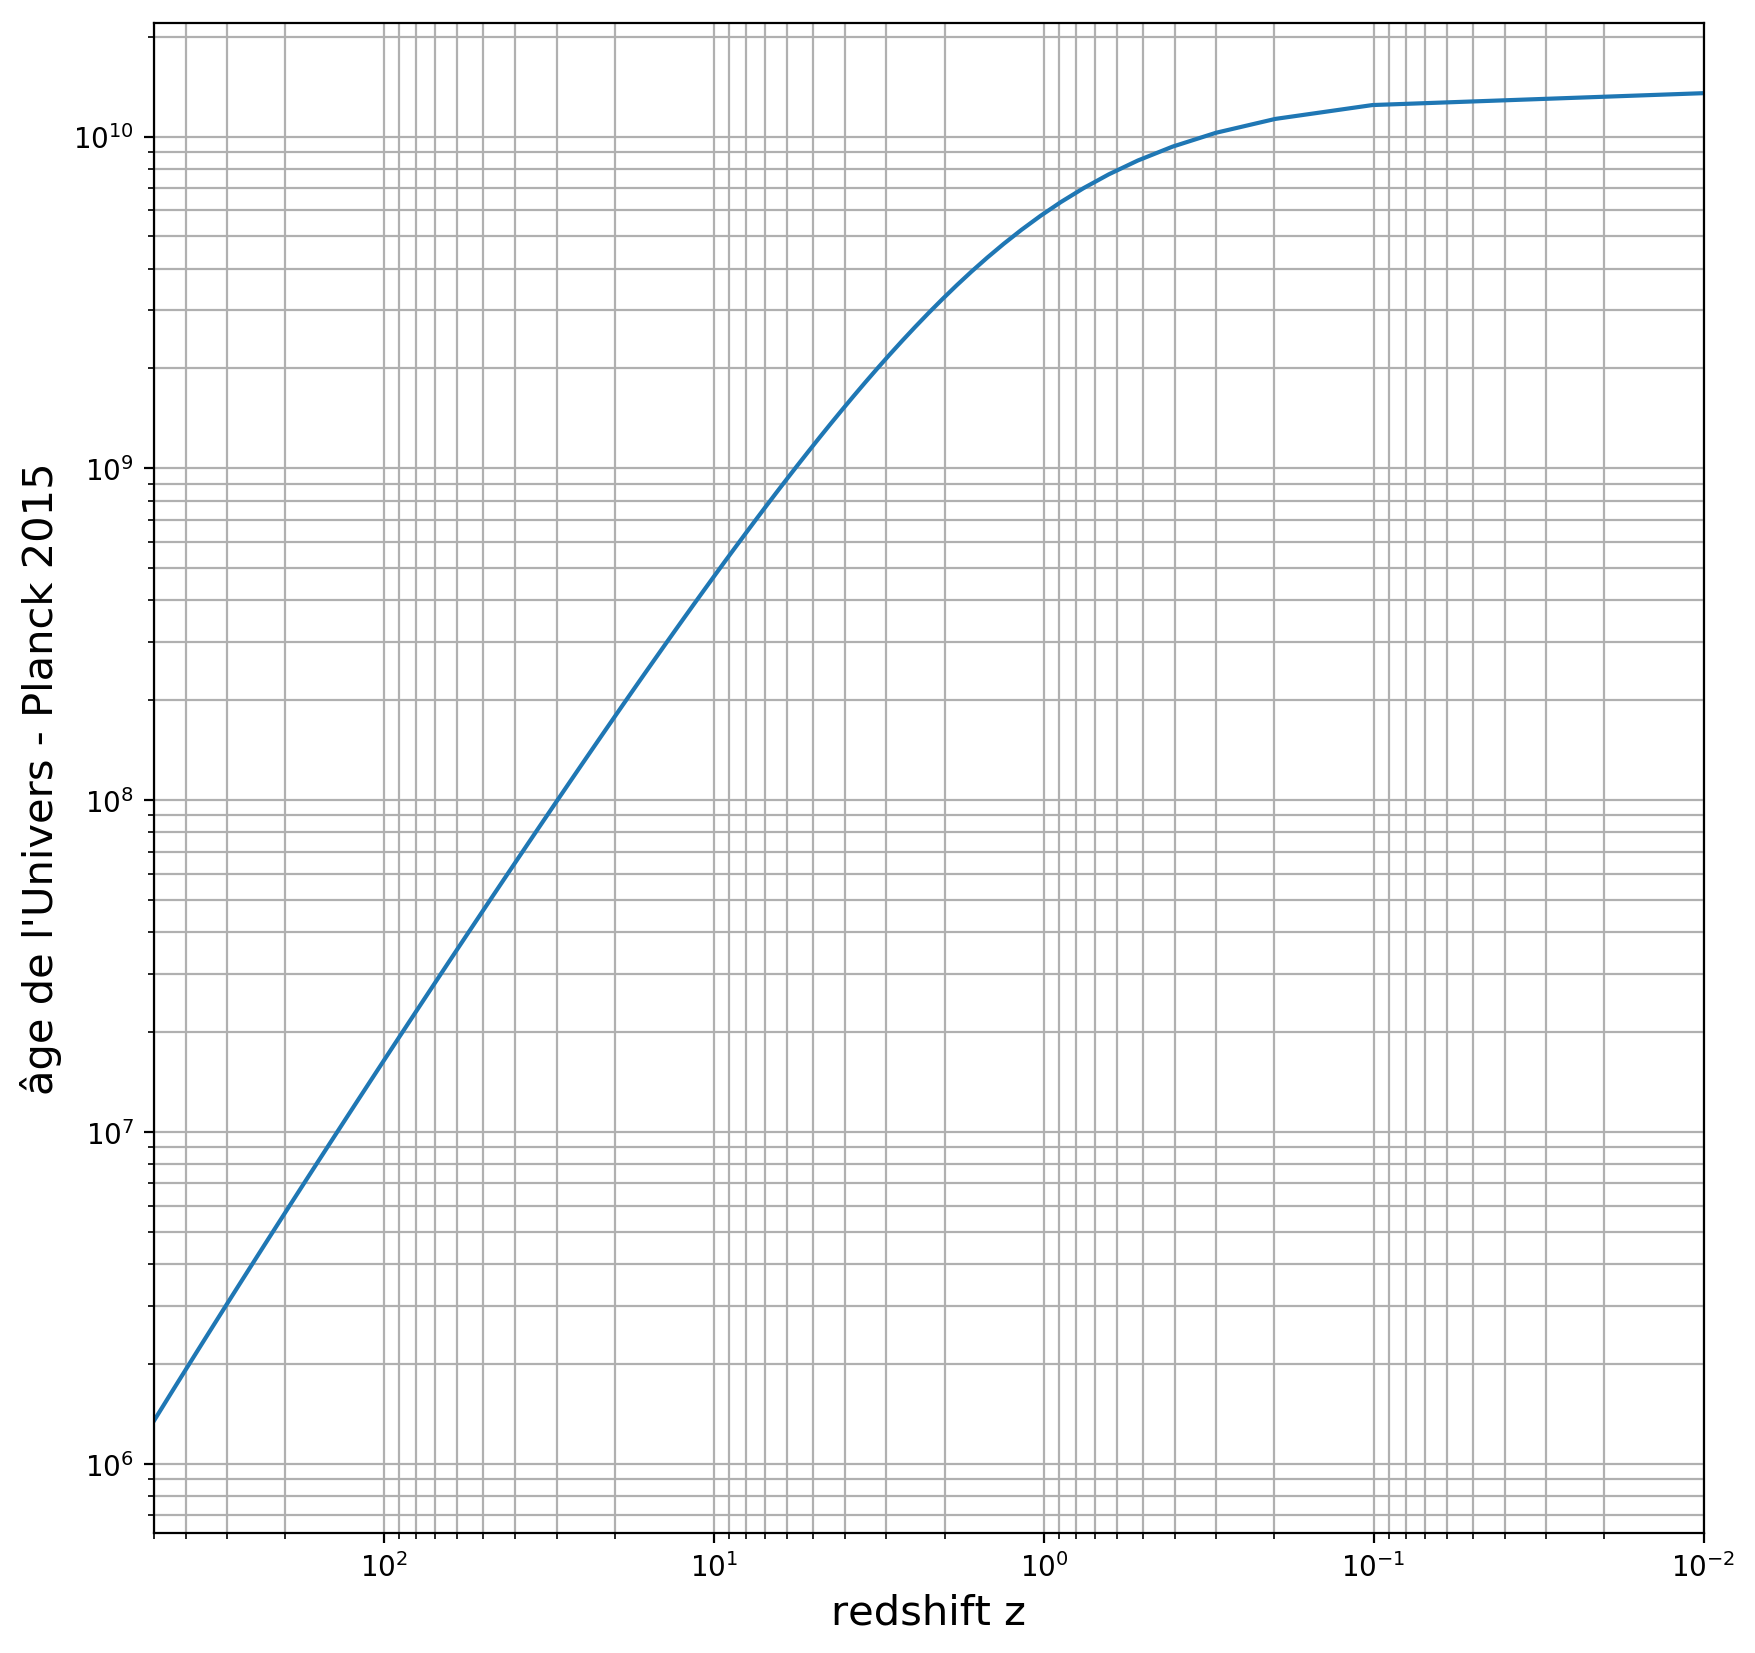
\includegraphics[height=12cm]{figs/zage.png}
	\caption[La relation redshift-age pour une cosmologie Planck 2015]{La relation entre l'âge de l'Univers (exprimé en années) et le redshift $z$ pour une cosmologie Planck 2015.}
	\label{f:zage}
\end{figure}

